\label{sec:5.9}

%%%%%%%%%%%%%%%%%%%%%%%%%%%%%%%%%%%%%%%%%%%%%%%%%%%
% Overflow wraparound
%%%%%%%%%%%%%%%%%%%%%%%%%%%%%%%%%%%%%%%%%%%%%%%%%%%

The gains of each stage are weighted by the calibration. If the sum of the weights of the stages is greater than $2^{16}$, then the digital correction logic can overflow, and a large input can lead to a small output code and vice versa. The stages were designed with an analog closed-loop gain slightly less than two. Based on supplied process data, we expected the closed-loop gain would be low enough to be free from overflow. In fact this was not the case and overflow was observed when the input voltage was close to one of the reference voltages. This can be seen in Figure~\ref{fig:adcoverflow}, which shows the response of the two different ADCs on one of the Cold ADC prototypes to the same input signal. The One the left portion of Figure~\ref{fig:adcoverflow} shows the ramp response of ADC0 and the prototype operates as expected. When the ADC is saturated, the digital output is pinned to its maximum value. On the right portion of Figure~\ref{fig:adcoverflow} overflow is observed as part of the ramp response of ADC1. In this case, the ADC input reaches its maximum value but instead of remaining pinned, the digital output jumps to a low value. This is due to higher-than-expected closed-loop gain in ADC1.
\begin{figure}[htb]
\centering
%\begin{minipage}[b]{1.0\textwidth}
\begin{center}
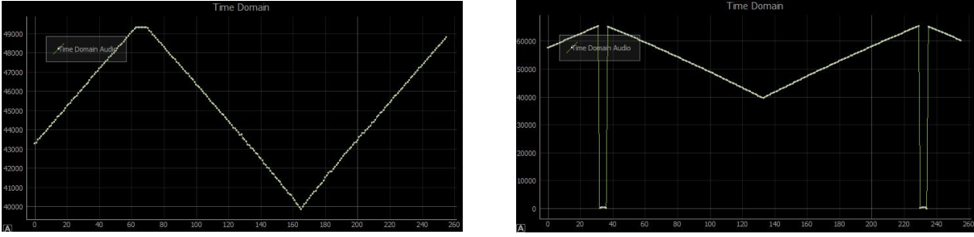
\includegraphics[width=1.0\textwidth]{figures/ADCOverflow.png}
\end{center}
%\end{minipage}
\caption{Digital overflow. The image on the left corresponds to ADC0 and the image on the right corresponds to ADC1.}
\label{fig:adcoverflow}
\end{figure}

We will fix this in two ways. First, we will further reduce the analog gain of the stages. Second, we will add to the next version of the prototype a digital overflow detection block that will sense over (or under) flow and pin the output code at a high or low level, respectively. It will do that by looking at the sign bit of the running sum one stage prior to the last. Then the algorithm will know whether to pin to a high or low value.
